\documentclass[12pt,a4paper]{article}
\usepackage[utf8]{inputenc}
\usepackage[german]{babel}
\usepackage[T1]{fontenc}
\usepackage{amsmath}
\usepackage{amsfonts}
\usepackage{amssymb}
\usepackage{graphicx}
\usepackage[left=3cm,right=3cm,top=3cm,bottom=3cm]{geometry}
\usepackage[table]{xcolor}
\setlength{\parskip}{3mm}
\setlength{\parindent}{0cm}
\author{Maike Meier and Lasse Schuirmann}
\title{Messtechnik und Messdatenverarbeitung - Blatt 7}
\newcommand*{\blankpage}{
  \vspace*{\fill}
  \begin{flushright}
  \tiny THIS PAGE INTENTIONALLY LEFT BLANK.
  \end{flushright}
  \pagebreak
}
\begin{document}
\rowcolors{2}{gray!25}{white}

\maketitle
\pagebreak

% See http://www.this-page-intentionally-left-blank.org/
\blankpage

\section*{Aufgabe 1}
\subsection*{1.1}
Um eine Ablösung des Sensors zu detektieren, kann der $\chi^2$-verteilung Anpassungstest durchgeführt werden.

Eine Voraussetzung für diesen Test ist, dass die Messwerte statistisch unabhängig sind und eine große Stichprobe vorhanden ist.

Der Test kann wie folgt durchgeführt werden:

\begin{enumerate}
\item Voraussetzungen sicherstellen
\item Klassen festlegen, Häufigkeiten $n_i$ bestimmen
\item Null- und Alternativhypothese aufstellen (ist normalverteilt/ist nicht normalverteilt)
\item Signifikanzniveau wählen
\end{enumerate}

\subsection*{1.2}
\scalebox{0.78}{
 \begin{tabular}{|r|c|c|c|c|c|c|c|c|}
 \hline
 \rowcolor{gray!50}
 Klasse & $\leq 35.0$ & $35.1 - 35.5$ & $35.6 - 36.0$ & $36.1 - 36.5$ & $36.6 - 37.0$ & $37.1 - 37.5$ & $37.6 - 38.0$ & $\geq 38.0$ \\
 Anzahl $n_i$ & $4$ & $9$ & $16$ & $20$ & $16$ & $16$ & $6$ & $8$ \\
 \hline
 \end{tabular}}

\noindent
\begin{minipage}{0.6\textwidth}
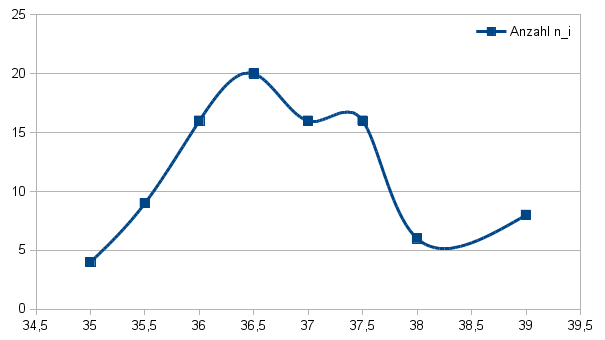
\includegraphics[scale=0.56]{1_2_diagram}
Diagramm 1.
\\
\end{minipage}
\begin{minipage}{0.4\textwidth}
Das Nebenstehende Diagramm ist eine Visualisierung der Obenstehenden Tabelle. (Hierbei wurde ein Datenpunkt jeweils bei einer Oberen Grenze der Klasse gezeichnet.)

Da jede Klasse nicht zu wenige Elemente enthält, das Diagramm aber aussagekräftig scheint, ist diese Einteilung bei dieser Stichprobenmenge sinnvoll.
\end{minipage}

\subsection*{1.3}
Die $p_i$s können mithilfe der gegebenen Daten aus einer Normalverteilung errechnet werden. Die gegebene Normalverteilungsfunktion ist im folgenden Diagramm dargestellt:

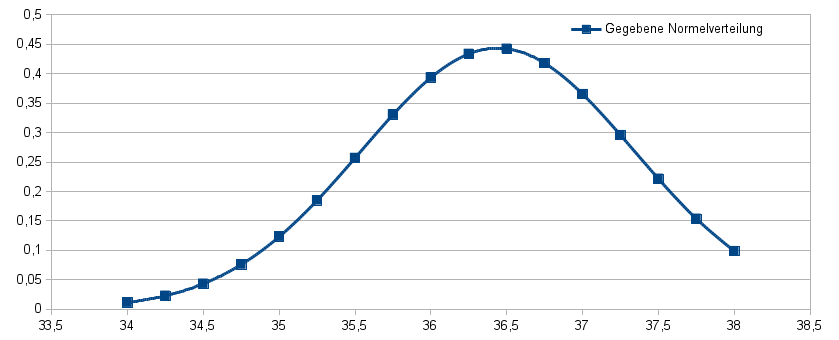
\includegraphics[scale=0.7]{1_3_normvert}

Ermittelt man die Werte der Dichtefunktion zu den gegebenen Klassengrenzen erhält man folgendes Diagramm:

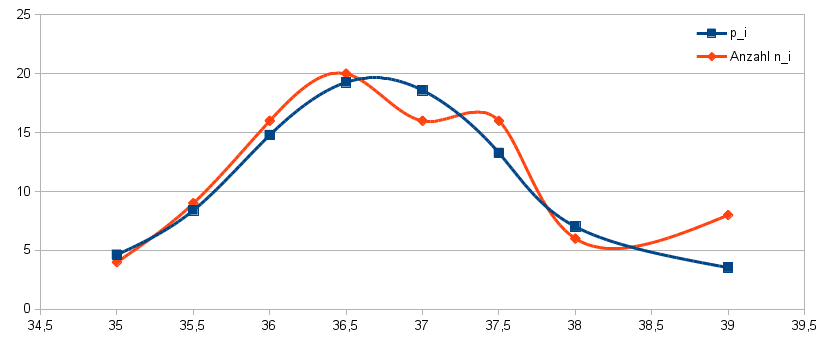
\includegraphics[scale=0.7]{1_3_dichte_vs_data}

Die dazugehörige Tabelle ist (Werte abgerundet [Informatiker] auf die erste Stelle nach dem Komma):

\scalebox{0.78}{
 \begin{tabular}{|r|c|c|c|c|c|c|c|c|}
 \hline
 \rowcolor{gray!50}
 Klasse & $\leq 35.0$ & $35.1 - 35.5$ & $35.6 - 36.0$ & $36.1 - 36.5$ & $36.6 - 37.0$ & $37.1 - 37.5$ & $37.6 - 38.0$ & $\geq 38.0$ \\
 Anzahl $n_i$ & $4$ & $9$ & $16$ & $20$ & $16$ & $16$ & $6$ & $8$ \\
 $p_i$ & $4.6$ & $8.4$ & $14.7$ & $19.2$ & $18.5$ & $13.2$ & $7.0$ & $3.5$ \\
 \hline
 \end{tabular}}
\subsection*{1.4}
\subsection*{1.5}

\end{document}